%% This is an example first chapter.  You should put chapter/appendix that you
%% write into a separate file, and add a line \include{yourfilename} to
%% main.tex, where `yourfilename.tex' is the name of the chapter/appendix file.
%% You can process specific files by typing their names in at the 
%% \files=
%% prompt when you run the file main.tex through LaTeX.


\chapter{The DGSPR design \& optimization}

As mentioned in the previous chapter, Bahrami et al. came up with an innovative design (the DGSPR sensor) that allows for multiple stable SPR modes which can consequently be used in multi-mode spectroscopy to combat many of the problems faced by regular SPR sensing. 

In this chapter, the novel DGSPR sensor will be examined in detail and the design parameters will be optimized with respect to operating \& manufacturing constraints. Whenever `DGSPR' is mentioned the structure discussed is identical to the one in \cite{farshid_ol}.

\section{The DGSPR design}

The DGSPR design that we will examine in this thesis will be the 3 mode spectroscopy variant (two p-polarized modes and one s-polarized mode). This should allow for the decoupling of $d_a$, $n_a$, and $n_b$ from each other. 

The DGSPR configuration consists of a SPR sensor affixed to a dielectric grating upon which targeted bio-receptors are placed. The metal (in this case gold was used) supports a p-polarized SPW whilst the dielectric gratings adds two more wave-guide modes (one p-polarized and the other s-polarized). Thus there are 3 real-time measures to solve for 3 different real-time parameters (we are naturally assuming linearity - see \autoref{SPR_var}; otherwise the problem might be intractable). Since we are only operating at a select wavelengths the dispersion characteristics are unimportant.

The DGSPR design is visible in  \autoref{fig:DGSPR}. It is important to note that in the following analysis, the depth of the gratings as seen in \autoref{fig:DGSPR} (a) are assumed to be infinite. This is a sufficiently good first order approximation. \footnote{One can argue that since we are assuming that the optical response is linear, analyzing the DGSPR structure in any greater detail than a first order approximation will not yield any significant gains in accuracy.}

\begin{figure}
\centering
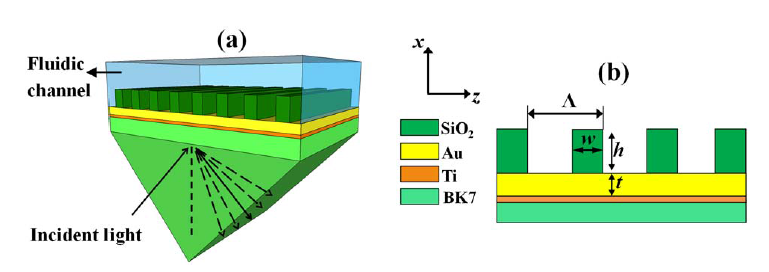
\includegraphics[width=0.75\textwidth]{DGSPR.png}
\caption{Figure showing the DGSPR sensor design as in \cite{farshid_ol}. In (a) you can see a 3D blue-print of the DSGPR sensor and in (b) you can see a 2D cross-section of the same sensor.}
\label{fig:DGSPR}
\end{figure}

There is an interesting emergent property of the dielectric gratings placed on top of the gold in the DGSPR. In cases where we are interested in analyte solutions that contain molecules of various different sizes (such as in blood), the dielectric grating acts as an inbuilt filter allowing one to separately study larger and smaller molecules simultaneously. More exactly we can say this: ``Molecules wider than $\Lambda - w$ will only be found at a height greater than $h$ from the gold surface (i.e. above the dielectric grating, in the bulk)''. This does not mean that smaller molecules do not exist in the bulk, only that larger molecules do not exist in the adlayer. 

\section{Simulation} \label{Sim}

The method used to simulate the DGSPR sensor was to model it using sensible first-order approximations to arrive at an approximate result. The accuracy of such an approximation then depends inversely on the step-size \footnote{The larger the step-size, the larger the second-order (and higher-order) contributions.} and it's immediately obvious that the run time of such a simulation is directly proportional to the step-size (inversely proportional to the accuracy). 

The first approximation is to consider the dielectric grating as a homogeneous medium with an average 	relative index as given in \cite{app_dig_opt}. The zeroth order effective medium theory approximation gives:

\begin{eqnarray} 
n_s = \sqrt{fn_1^2 + (1-f)n_2^2} \label{EMT1}\\
n_p = \frac{1}{\sqrt{\frac{f}{n_1^2} + \frac{1-f}{n_2^2}}} \label{EMT2}
\end{eqnarray}

Where $n_1$ and $n_2$ are the indexes of the alternating slabs of dielectric that constitute the grating (with periodicity $\Lambda$), and $f$ is the volume fraction of the material with index $n_1$ (in this case $f = \frac{w}{\Lambda}$). 

Using \autoref{EMT1} \& \autoref{EMT2}, we may replace the grating structure with a simple dielectric with a constant index($n_{eff}$). This simplifies the DGSPR into a SPR, but one that can support two modes (similar to the Plasmon Wave-guide Resonance bio-sensor as discussed in \cite{farshid_conf}). 

In using the zeroth order approximation we ignore the influence of the gratings. This can be remedied by using Rigorous-Coupled Wave Analysis RCWA) to simulate the grating structure. In applying RCWA we end up right where we started, with an approximation that can support three modes. 

To analyze the effectiveness of a particular configuration when applied to bio-sensing, we need a figure of merit (FoM) which in this case is defined by Bahrami et al. in \cite{farshid_ol} as:

\begin{eqnarray}\label{FOM}
CSF = SF \times SM \\
FoM = CSF^{p1}_{surf,thick} \times CSF^{p2}_{surf,thick} \times CSF^{s}_{bulk,index}
\end{eqnarray}

Where SM is the sensor merit, and SF is the sensor's sensitivity factor. The Combined Sensitivity Factor (CSF) is inversely proportional to the sensor's limit of detection. Thus it follows that the better the sensor, the larger the CSF. \footnote{The CSF is in essence of how `sharp' the sensor's resonance is, and can be calculated as the ratio of the resonance depth \& the resonance FWHM. An in depth explanation of the definition of CSF is available in \cite{CSF_def}.}

\subsection{Simulation Code}

The simulation code was written in FORTRAN 90 (this is the same code used by Farshid et al. in \cite{farshid_ol}) and the simulation method roughly follows the pseudo-code shown in \autoref{Code: main} and \autoref{Code: support}.

\begin{figure}
%\centering
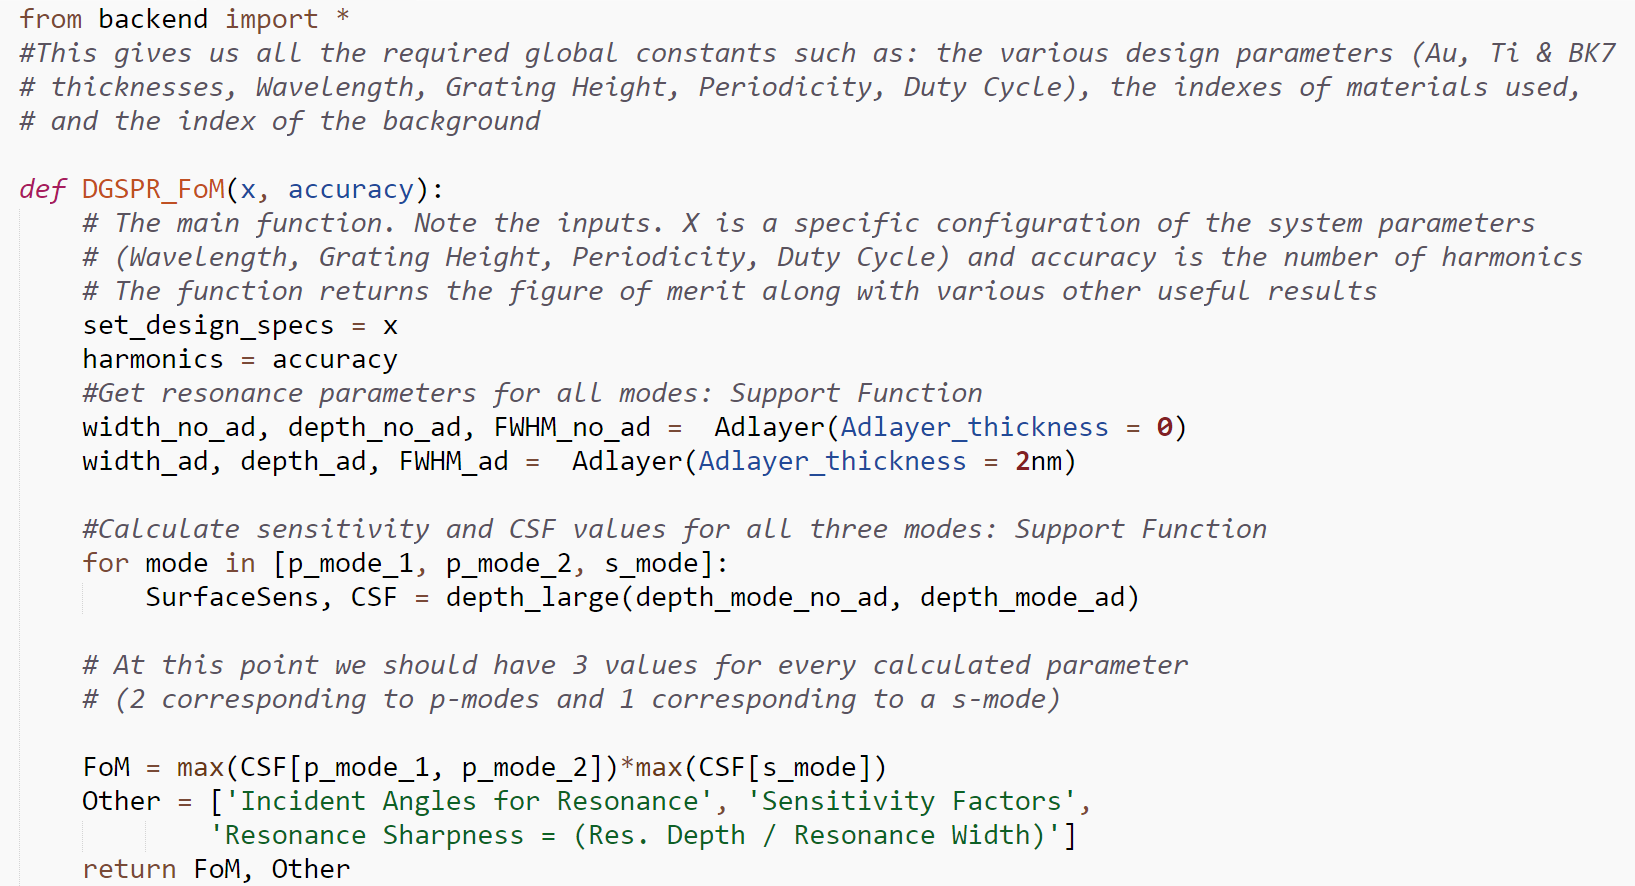
\includegraphics[width=1.1\textwidth]{main_white.png}
\caption{Pythonic pseudo-code implementation of the integral aspects that comprise the DGSPR simulation}
\label{Code: main}
\end{figure}

\begin{figure}
%\centering
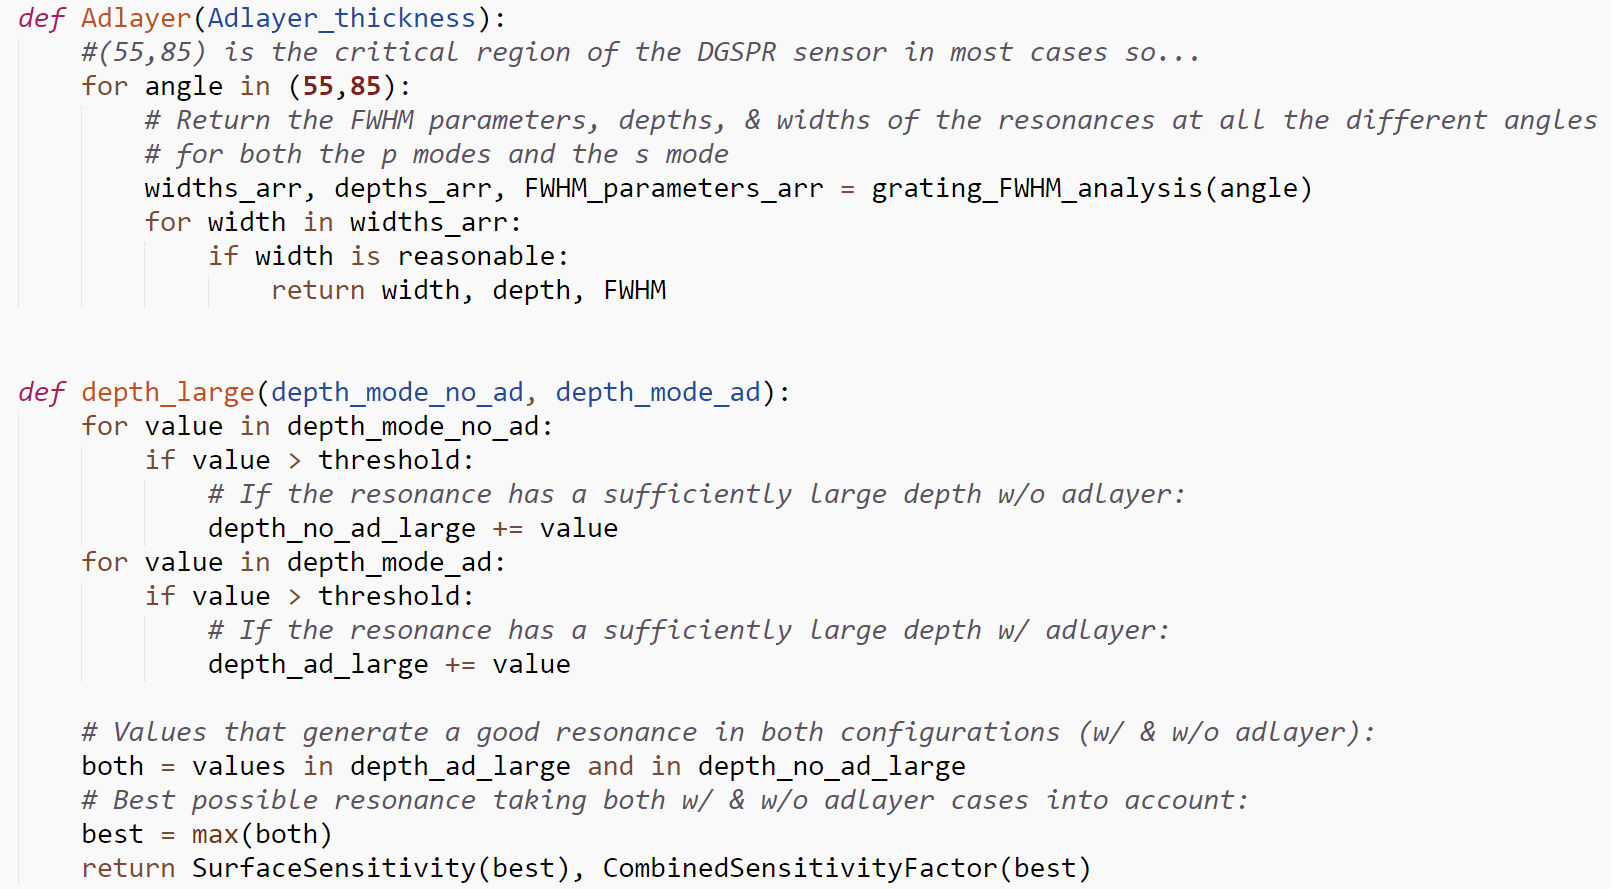
\includegraphics[width=1.1\textwidth]{support_white.png}
\caption{Pythonic pseudo-code implementation of the support code called from the main function \ref{Code: main}}
\label{Code: support}
\end{figure}

There are a few things to keep in mind when reading this pseudo-code. In writing the code we have assumed infinitely deep gratings (in the y-direction in \autoref{fig:DGSPR}), and an infinitely thick background. 

Additionally, it should be mentioned that it is perfectly alright to have 3 different resonance angles (one for the s-mode and two for the p-modes) - this is not an expensive operation, and the system can be operated at 3 angles without any significant cost.

\section{Optimization}

The optimization of the DGSPR design is done by using methods disclosed in \autoref{Sim}, and is aimed at maximizing the FoM defined in \autoref{FOM}.

However, beyond the FoM, we also have to consider whether or not the final DGSPR sensor can be manufactured. This imposes certain additional criteria that we must recognize. It is also important to note that a DGSPR sensor must be comparable to a SPR sensor and as such, the values for the CSF-p and CSF-s must be atleast on the same order as those for an SPR sensor as given in \cite{farshid_ol}.

For a given set $X$ consisting of $N$ different DGSPR configurations, the optimization of the design can be broken down into three sequential processes. Firstly, there is the low-accuracy analysis of all configurations in $X$. It is succeeded by the mid-accuracy analysis of select configurations that look promising. Finally we have the extremely accurate analysis of less than 3 configurations to select the best configuration in $X$.

Initially the optimization was done using genetic algorithms, but this was later found to be unfeasible due to a large majority of the results not being easily and/or cheaply manufacturable. Instead, the results of the genetic algorithm optimization process were used to constrain the parameter space for an exhaustive brute-force search. The constrained space obeyed the following rules:

\begin{itemize}
\item The wavelength was between $700 nm$ and $1500 nm$ (usually around $770 nm$).\\
\item The duty cycle $\frac{w}{\Lambda}$ was less than $0.55$. \\
\item The grating period $\Lambda$ was less than $1500 nm$. \\
\item The grating height $h$ was less than $3 \mu m$. 
\end{itemize}

In this way the parameter/design space was reduced to a much more manageable number of configurations ($\sim$ 10,000). Each configuration was then examined in turn in order to find the global optima.  


\subsection{Manufacturing considerations}

Whilst the FoM characterizes the DGSPR sensor, some of the `good' configurations output by a genetic algorithm based optimization routine are completely unfeasible due to not being manufacturable. Consequently, based on conversations with manufacturing companies specializing in Nano-Electro-Mechanical Systems (NEMS), a few general guidelines were devised: \footnote{The cost of manufacturing the DGSPR sensor was also taken into account when devising the general guidelines.}

\begin{itemize}
\item The height ($h$) of the gratings should increase in multiples of 500$nm$.

\item The width ($w$) and the periodicity ($\Lambda$) of the gratings should be multiples of 100 $nm$. 

\item If $w$ and $\Lambda$ cannot be multiples of 100 $nm$, then selecting them as multiples of 50 $nm$ is a viable, but less favorable, alternative. 
\end{itemize}

\subsection{Low Accuracy Mass Analysis}

In the Low Accuracy Mass Analysis of many different combinations of grating period ($\Lambda$) and duty cycle ($\frac{w}{\Lambda}$), the accuracy was set to 2 harmonic orders. Furthermore, the FoM was modified such that it was 0 if it was not comparable to the SPR sensor or if the sensor did not support atleast 3 modes (2 p \& 1 s). $\lambda$ was set to be $770 nm$.

The period increased by 100 $nm$ between iterations, and the duty cycle varied between 0.1 and 0.9 in every iteration. All other variables such as grating height or incident wavelength were kept constant. 

This was repeated for grating heights in \{1.0 $\mu m$, 1.5 $\mu m$, 2.0 $\mu m$ \} - the grating height stepping size is 500 $nm$, adhering to the general guidelines from before. The five best configurations corresponding to each grating height value were taken and analyzed further at a higher level of accuracy. \footnote{Examining the top two peaks would have been sufficient.}

This resulted in graphs such as those in \autoref{fig:low1} \& \autoref{fig:low2}.

\begin{figure}
\centering
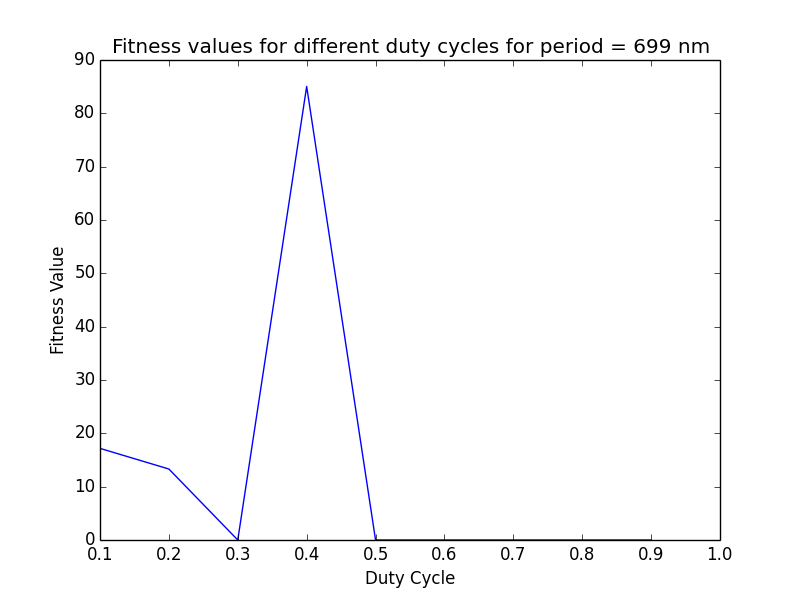
\includegraphics[width=0.75\textwidth]{low1.png}
\caption{Figure showing some examples of the results of low accuracy mass analysis with $h$ = 1.5 $\mu m$, $t_{Au}$ = 50 $nm$}
\label{fig:low1}
\end{figure}

\begin{figure}
\centering
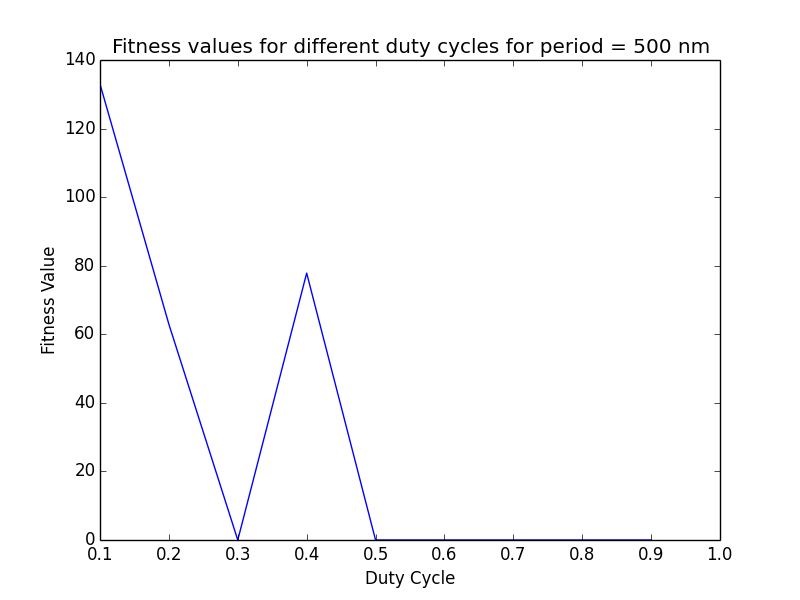
\includegraphics[width=0.75\textwidth]{low2.png}
\caption{Figure showing more examples of the results of low accuracy mass analysis with $h$ = 1.5 $\mu m$, $t_{Au}$ = 50 $nm$}
\label{fig:low2}
\end{figure}

\subsection{Mid Accuracy Select Analysis}

In the Mid Accuracy Select Analysis of select combinations of grating period ($\Lambda$), duty cycle ($\frac{w}{\Lambda}$), and grating height $h$ \footnote{At this point it is interesting to note that exhaustive testing of configurations revealed that the other parameters identified by the genetic algorithm approach in \cite{farshid_ol} worked very well and there was no reason to deviate from them significantly. Indeed $t_{Au}$ = 50 $nm$ turned out to be the best possible value for most configurations. However, the incident wavelength did need some tuning.} the accuracy was set to 6 harmonic orders. 

The previous modification to the FoM [it was 0 if it was not comparable to the SPR sensor or if the sensor did not support atleast 3 modes (2 p \& 1 s)] was still used.

As stated earlier, the five best configurations corresponding to every value of grating height (as measured by FoM), were selected to be analyzed at mid-accuracy. For each configuration, the incident wavelength was varied so as to select the optimum operating wavelength for the DGSPR sensor. After the operating wavelength was identified, the duty cycle was perturbed slightly so as to get $w$ to be a multiple of 100 $nm$ or atleast a multiple of 50 $nm$. 

The best three configurations (which are alike in every way but for different duty cycles) were then taken forward to be analyzed at extremely high accuracy. 

Mid-accuracy select analysis resulted in graphs such as those in \autoref{fig:mid1}, \autoref{fig:mid2}, and \autoref{fig:mid3}.

\begin{figure}
\centering
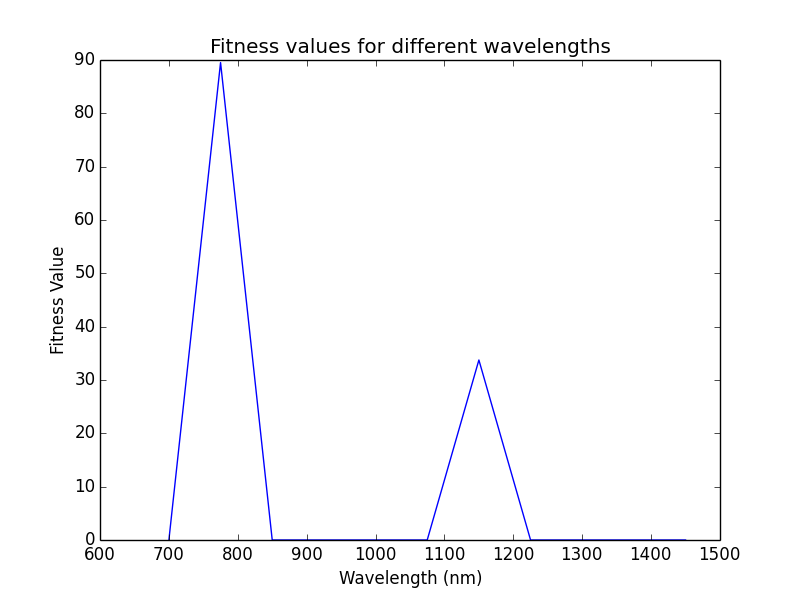
\includegraphics[width=0.75\textwidth]{mid1.png}
\caption{Figure showing some examples of the results of mid accuracy analysis with $h$ = 1.5 $\mu m$, $\Lambda$ = 1200 $nm$, $t_{Au}$ = 50 $nm$ and $\frac{w}{\Lambda}$ = 0.2}
\label{fig:mid1}
\end{figure}

\begin{figure}
\centering
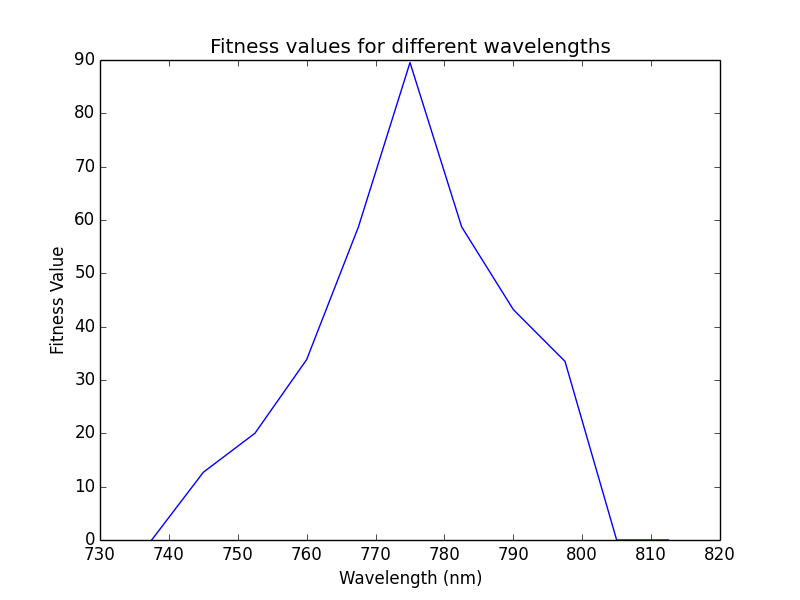
\includegraphics[width=0.75\textwidth]{mid2.png}
\caption{Figure showing more examples of the results of mid accuracy analysis with $h$ = 1.5 $\mu m$, $\Lambda$ = 1200 $nm$, $t_{Au}$ = 50 $nm$ and $\frac{w}{\Lambda}$ = 0.2}
\label{fig:mid2}
\end{figure}

\begin{figure}
\centering
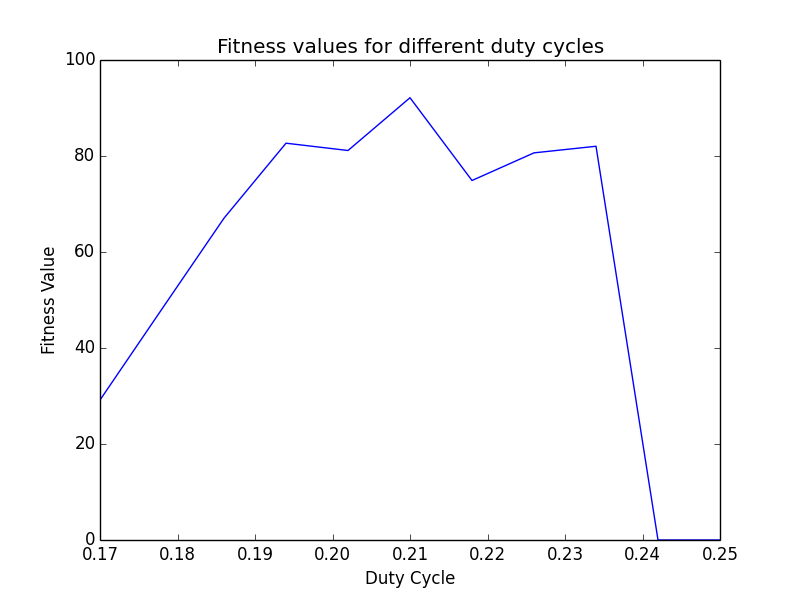
\includegraphics[width=0.75\textwidth]{mid3.png}
\caption{Figure showing even more examples of the results of mid accuracy analysis with $h$ = 1.5 $\mu m$, $\Lambda$ = 1200 $nm$, $t_{Au}$ = 50 $nm$ and $\frac{w}{\Lambda}$ = 0.2}
\label{fig:mid3}
\end{figure}


\subsection{Extremely High Accuracy Analysis}

In the Extremely High Accuracy Analysis of select combinations of grating period ($\Lambda$), duty cycle ($\frac{w}{\Lambda}$), and grating height $h$, the accuracy was set to 10 harmonic orders. The previous modification to the FoM still applied.

This step is not so much to get the best possible configuration possible, as it is to get reliable FoM values for a given configuration. \footnote{Reliability comes at a large cost - each configuration took about 10 minutes to run on an i5 with 4GB RAM.} The best three configurations are then compared against each other and the best configuration is selected.

High Accuracy Analysis basically resulted in trustworthy FoM numbers. 

\subsection{Results \& Optimized Design}

It is important to remember that this method of optimization will only provide local maxima for the FoM within the constrained design/parameter space. That is, all configurations that make it to the Extremely High Accuracy Analysis stage are the best configurations (constrained in the ways mentioned previously) within a certain neighborhood in the DGSPR parameter space. But, by comparing various local maxima to each other, if an exhaustive search of the constrained parameter space has been completed, one can be reasonably sure that the largest maxima is a global maxima.

The results of the High Accuracy Analysis are conglomerated in \autoref{table:res_anal} 

% Please add the following required packages to your document preamble:
% \usepackage{booktabs}
% \usepackage{graphicx}
\begin{table}[h]
\centering
\resizebox{\textwidth}{!}{%
\begin{tabular}{@{}llllll@{}}
\toprule
\textbf{Grating Height ($\mu m$)} & \textbf{Incident Wavelength ($nm$)} & \textbf{Grating Period ($nm$)} & \textbf{Duty Cycle} & \textbf{Grating Width ($nm$)} & \textbf{FoM} \\ \midrule
1.5                          & 775                               & 1200                         & 0.20833             & 250                         & 88.25143     \\
1.5                          & 782.5                             & 1200                         & 0.416667            & 500                         & 99.445       \\
2.0                          & 760                               & 1000                         & 0.3                 & 300                         & 199.8923     \\
2.0                          & 787                               & 500                          & 0.5                 & 250                         & 32.09551     \\
1.0                          & 790                               & 500                          & 0.2                 & 100                         & 133.8602     \\ \bottomrule
\end{tabular}
}
\caption{Table showing the results of the High Accuracy Analysis i.e. the best possible configurations of the sensor for manufacturing}
\label{table:res_anal}
\end{table}

The third configuration ($h$ = 2.0, $\Lambda$ = 1000 $nm$, and $w$ = 300 $nm$) seems to be the global maxima and is what we will be discussing henceforth. It shall be known as the optimized design.

\section{Summary}

In this chapter a brief introduction to the DGSPR sensor, along with its design considerations, was provided. The method used to simulate the DGSPR was also explained and the optimization process was discussed in detail. Finally, an optimized design was discovered by creating a fully spanning atlas of the design space using various localized maps. The next chapter will deal with the manufacturing methods used in the NEMS industry and will also decide which method should be used to actually manufacture the optimized design. 
